% Options for packages loaded elsewhere
\PassOptionsToPackage{unicode}{hyperref}
\PassOptionsToPackage{hyphens}{url}
\PassOptionsToPackage{dvipsnames,svgnames,x11names}{xcolor}
%
\documentclass[
]{agujournal2019}

\usepackage{amsmath,amssymb}
\usepackage{iftex}
\ifPDFTeX
  \usepackage[T1]{fontenc}
  \usepackage[utf8]{inputenc}
  \usepackage{textcomp} % provide euro and other symbols
\else % if luatex or xetex
  \usepackage{unicode-math}
  \defaultfontfeatures{Scale=MatchLowercase}
  \defaultfontfeatures[\rmfamily]{Ligatures=TeX,Scale=1}
\fi
\usepackage{lmodern}
\ifPDFTeX\else  
    % xetex/luatex font selection
\fi
% Use upquote if available, for straight quotes in verbatim environments
\IfFileExists{upquote.sty}{\usepackage{upquote}}{}
\IfFileExists{microtype.sty}{% use microtype if available
  \usepackage[]{microtype}
  \UseMicrotypeSet[protrusion]{basicmath} % disable protrusion for tt fonts
}{}
\makeatletter
\@ifundefined{KOMAClassName}{% if non-KOMA class
  \IfFileExists{parskip.sty}{%
    \usepackage{parskip}
  }{% else
    \setlength{\parindent}{0pt}
    \setlength{\parskip}{6pt plus 2pt minus 1pt}}
}{% if KOMA class
  \KOMAoptions{parskip=half}}
\makeatother
\usepackage{xcolor}
\setlength{\emergencystretch}{3em} % prevent overfull lines
\setcounter{secnumdepth}{-\maxdimen} % remove section numbering
% Make \paragraph and \subparagraph free-standing
\ifx\paragraph\undefined\else
  \let\oldparagraph\paragraph
  \renewcommand{\paragraph}[1]{\oldparagraph{#1}\mbox{}}
\fi
\ifx\subparagraph\undefined\else
  \let\oldsubparagraph\subparagraph
  \renewcommand{\subparagraph}[1]{\oldsubparagraph{#1}\mbox{}}
\fi


\providecommand{\tightlist}{%
  \setlength{\itemsep}{0pt}\setlength{\parskip}{0pt}}\usepackage{longtable,booktabs,array}
\usepackage{calc} % for calculating minipage widths
% Correct order of tables after \paragraph or \subparagraph
\usepackage{etoolbox}
\makeatletter
\patchcmd\longtable{\par}{\if@noskipsec\mbox{}\fi\par}{}{}
\makeatother
% Allow footnotes in longtable head/foot
\IfFileExists{footnotehyper.sty}{\usepackage{footnotehyper}}{\usepackage{footnote}}
\makesavenoteenv{longtable}
\usepackage{graphicx}
\makeatletter
\def\maxwidth{\ifdim\Gin@nat@width>\linewidth\linewidth\else\Gin@nat@width\fi}
\def\maxheight{\ifdim\Gin@nat@height>\textheight\textheight\else\Gin@nat@height\fi}
\makeatother
% Scale images if necessary, so that they will not overflow the page
% margins by default, and it is still possible to overwrite the defaults
% using explicit options in \includegraphics[width, height, ...]{}
\setkeys{Gin}{width=\maxwidth,height=\maxheight,keepaspectratio}
% Set default figure placement to htbp
\makeatletter
\def\fps@figure{htbp}
\makeatother

\usepackage{url} %this package should fix any errors with URLs in refs.
\usepackage{lineno}
\usepackage[inline]{trackchanges} %for better track changes. finalnew option will compile document with changes incorporated.
\usepackage{soul}
\linenumbers
\makeatletter
\@ifpackageloaded{caption}{}{\usepackage{caption}}
\AtBeginDocument{%
\ifdefined\contentsname
  \renewcommand*\contentsname{Table of contents}
\else
  \newcommand\contentsname{Table of contents}
\fi
\ifdefined\listfigurename
  \renewcommand*\listfigurename{List of Figures}
\else
  \newcommand\listfigurename{List of Figures}
\fi
\ifdefined\listtablename
  \renewcommand*\listtablename{List of Tables}
\else
  \newcommand\listtablename{List of Tables}
\fi
\ifdefined\figurename
  \renewcommand*\figurename{Figure}
\else
  \newcommand\figurename{Figure}
\fi
\ifdefined\tablename
  \renewcommand*\tablename{Table}
\else
  \newcommand\tablename{Table}
\fi
}
\@ifpackageloaded{float}{}{\usepackage{float}}
\floatstyle{ruled}
\@ifundefined{c@chapter}{\newfloat{codelisting}{h}{lop}}{\newfloat{codelisting}{h}{lop}[chapter]}
\floatname{codelisting}{Listing}
\newcommand*\listoflistings{\listof{codelisting}{List of Listings}}
\makeatother
\makeatletter
\makeatother
\makeatletter
\@ifpackageloaded{caption}{}{\usepackage{caption}}
\@ifpackageloaded{subcaption}{}{\usepackage{subcaption}}
\makeatother
\ifLuaTeX
  \usepackage{selnolig}  % disable illegal ligatures
\fi
\usepackage{bookmark}

\IfFileExists{xurl.sty}{\usepackage{xurl}}{} % add URL line breaks if available
\urlstyle{same} % disable monospaced font for URLs
\hypersetup{
  pdftitle={Slide Decks for John Curtin's Scientific Presentations},
  pdfauthor={John J. Curtin},
  colorlinks=true,
  linkcolor={blue},
  filecolor={Maroon},
  citecolor={Blue},
  urlcolor={Blue},
  pdfcreator={LaTeX via pandoc}}


\draftfalse

\begin{document}
\title{Slide Decks for John Curtin's Scientific Presentations}

\authors{John J. Curtin\affil{1}}
\affiliation{1}{Department of Psychology, University of
Wisconsin-Madison, }
\correspondingauthor{John J. Curtin}{jjcurtin@wisc.edu}






\subsection{Overview}\label{overview}

\subsection{Generic}\label{generic}

\subsection{Burden Study}\label{burden-study}

\subsection{EMA Study}\label{ema-study}

\subsubsection{Figures}\label{figures}

\begin{figure}[H]

\centering{

\captionsetup{labelsep=none}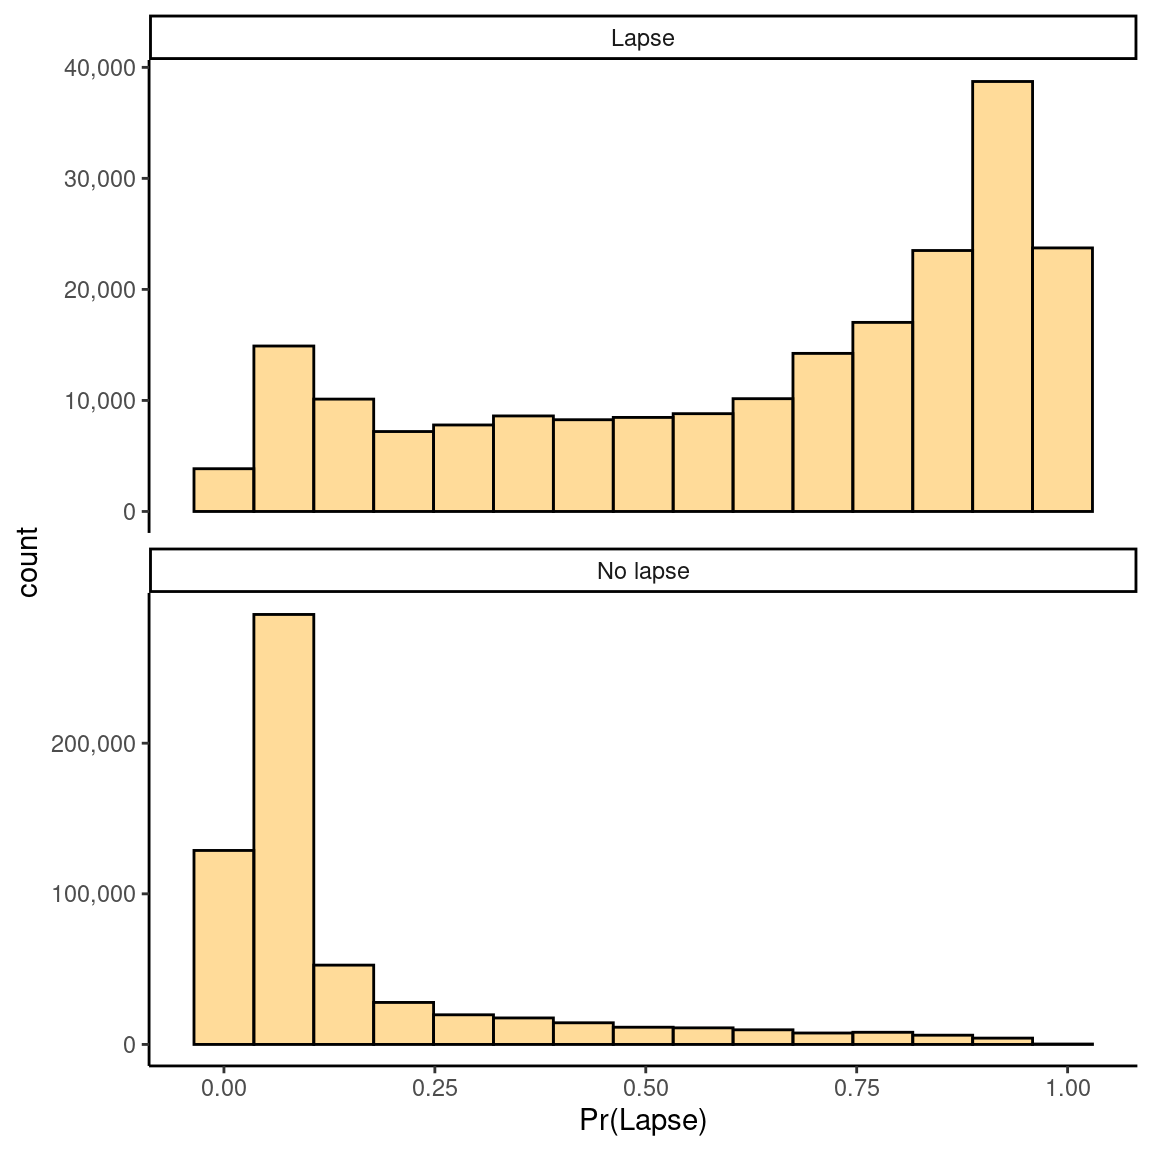
\includegraphics{index_files/figure-latex/notebooks-ema_figs_probability-fig-week-no_dec_thres-output-1.png}

}

\caption{\label{fig-week-no_dec_thres}}

\end{figure}%

\textsubscript{Source:
\href{https://jjcurtin.github.io/lectures_science/notebooks/ema_figs_probability-preview.html\#cell-fig-week-no_dec_thres}{Risk1
probability plots}}

\begin{figure}[H]

\centering{

\captionsetup{labelsep=none}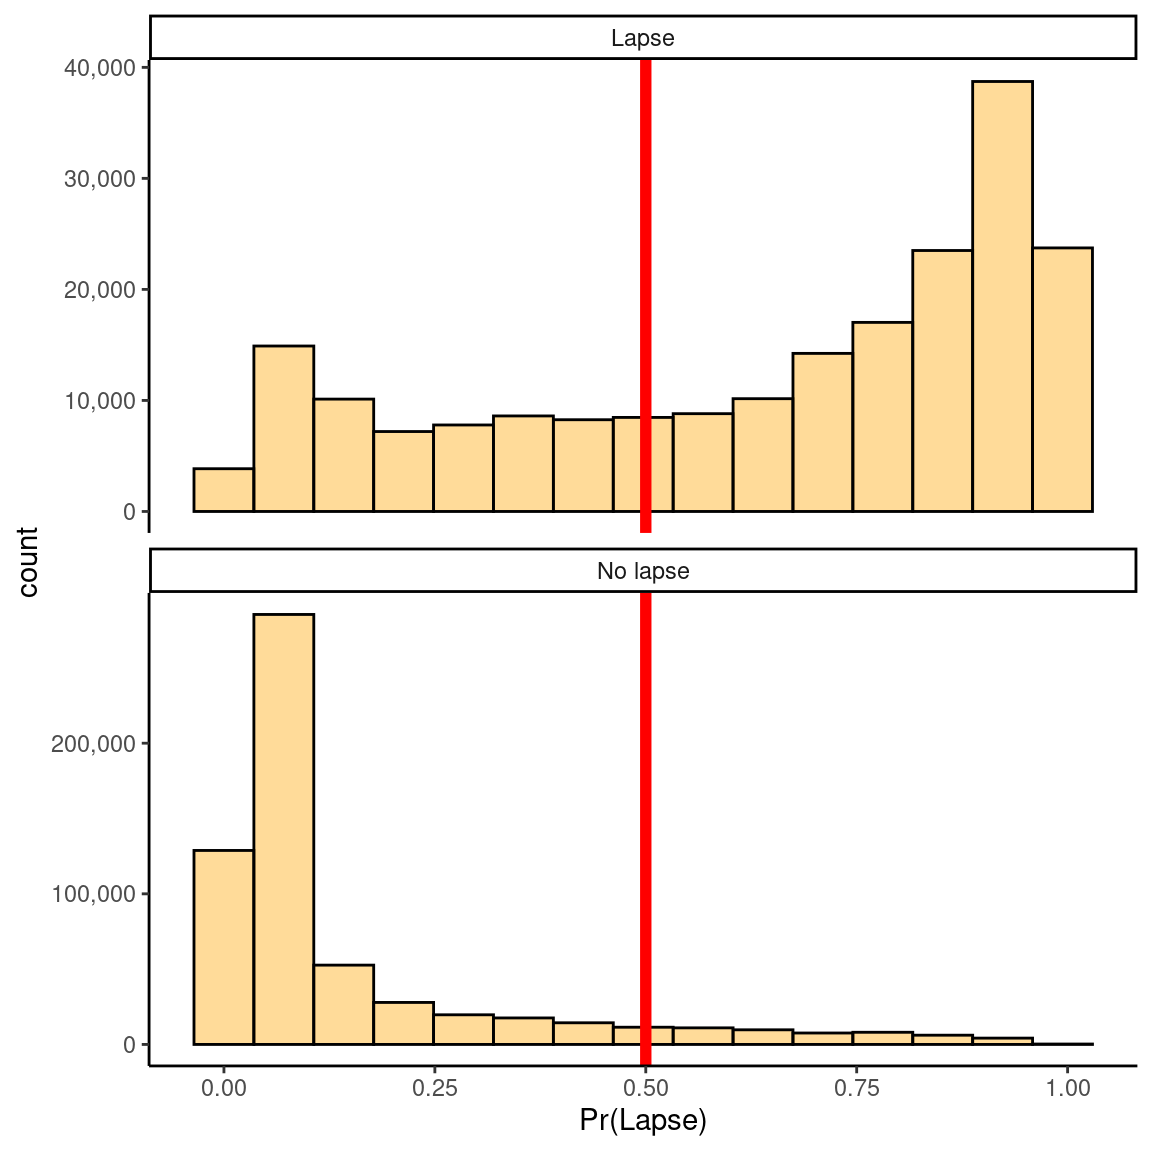
\includegraphics{index_files/figure-latex/notebooks-ema_figs_probability-fig-week-output-2.png}

}

\caption{\label{fig-week}}

\end{figure}%

\textsubscript{Source:
\href{https://jjcurtin.github.io/lectures_science/notebooks/ema_figs_probability-preview.html\#cell-fig-week}{Risk1
probability plots}}

\begin{figure}[H]

\centering{

\captionsetup{labelsep=none}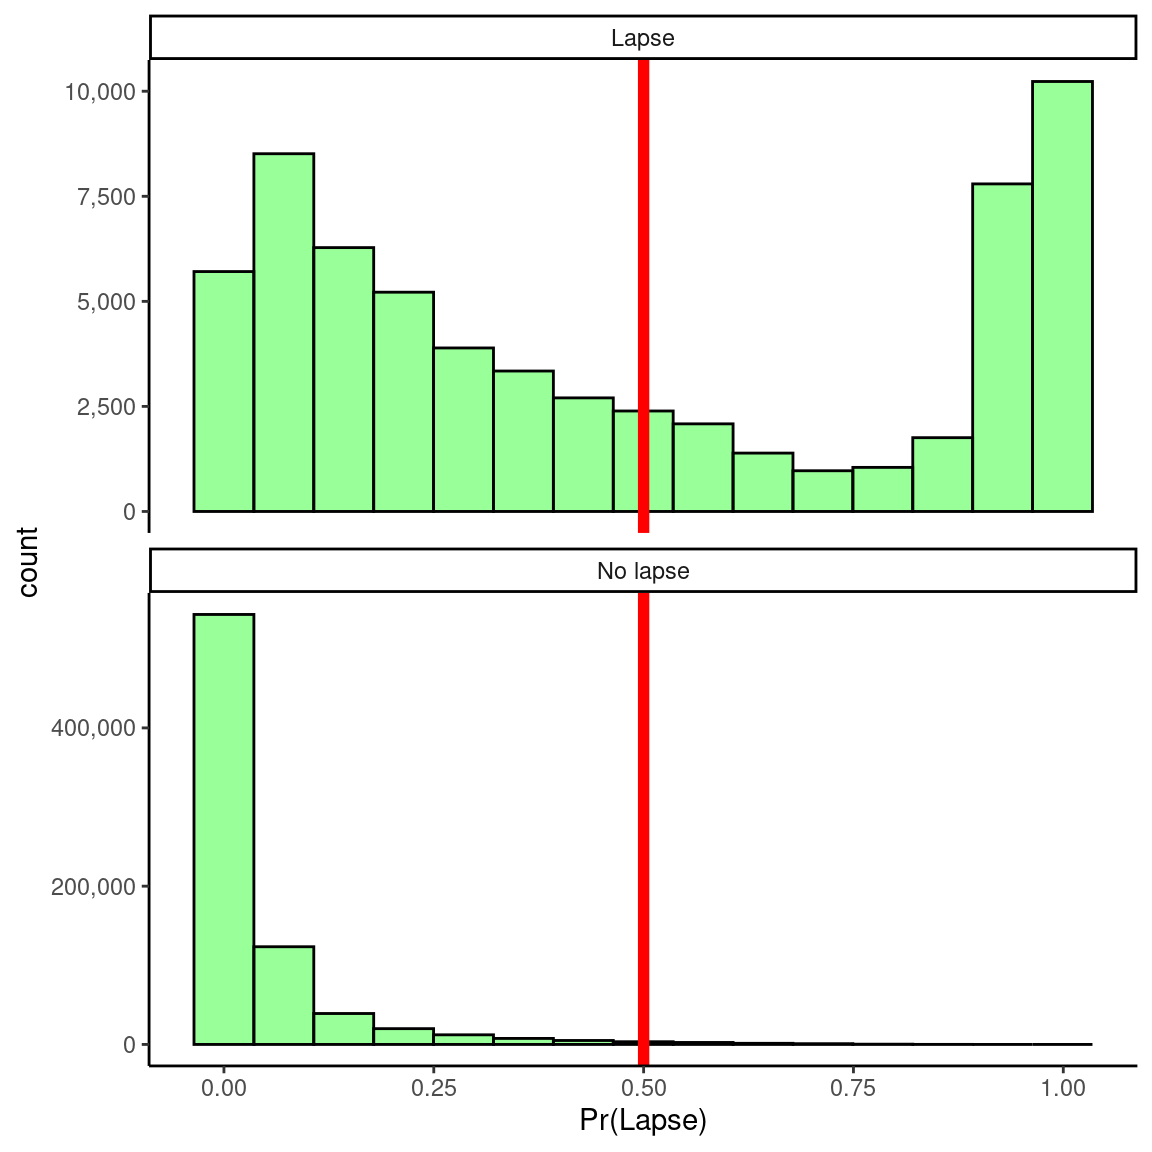
\includegraphics{index_files/figure-latex/notebooks-ema_figs_probability-fig-day-output-1.png}

}

\caption{\label{fig-day}}

\end{figure}%

\textsubscript{Source:
\href{https://jjcurtin.github.io/lectures_science/notebooks/ema_figs_probability-preview.html\#cell-fig-day}{Risk1
probability plots}}

\begin{figure}[H]

\centering{

\captionsetup{labelsep=none}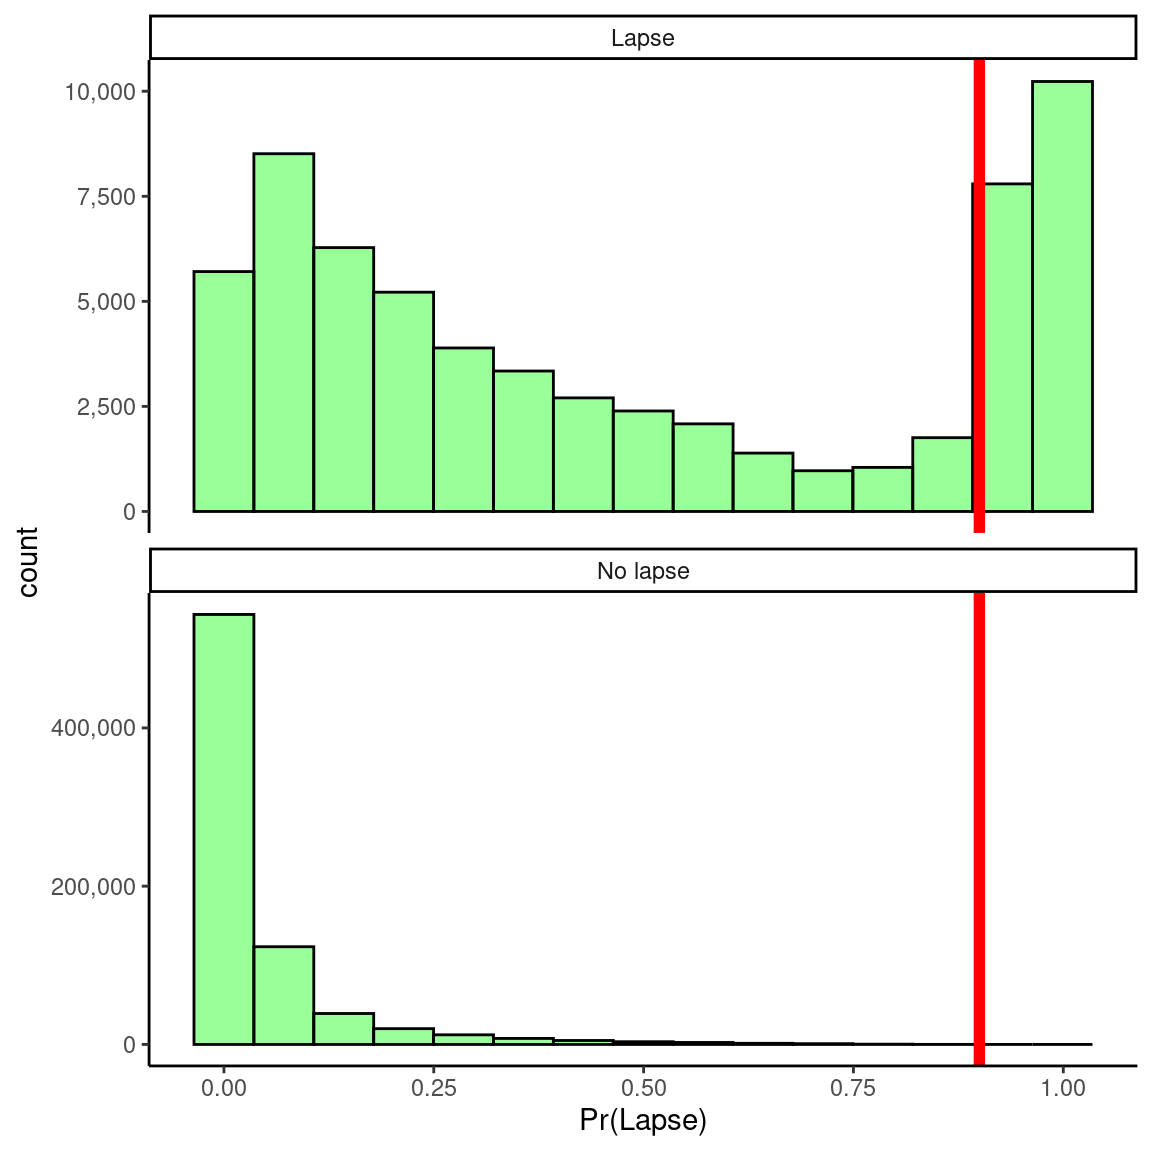
\includegraphics{index_files/figure-latex/notebooks-ema_figs_probability-fig-day-high_dec_thres-output-1.png}

}

\caption{\label{fig-day-high_dec_thres}}

\end{figure}%

\textsubscript{Source:
\href{https://jjcurtin.github.io/lectures_science/notebooks/ema_figs_probability-preview.html\#cell-fig-day-high_dec_thres}{Risk1
probability plots}}

\subsubsection{Tables}\label{tables}

\phantomsection\label{table-paper}
\begin{longtable}[]{@{}llll@{}}
\caption{Areas under the receiver operating characteristic curves
(auROCs) summarize the model's sensitivity and specificity over all
possible decision thresholds. Sensitivity, specificity, balanced
accuracy, positive predictive value, and negative predictive value are
performance metrics calculated at a single decision threshold for each
model determined with Youden's index. All metrics represent median
values across 30 held-out test sets.}\tabularnewline
\toprule\noalign{}
Metric & Week & Day & Hour \\
\midrule\noalign{}
\endfirsthead
\toprule\noalign{}
Metric & Week & Day & Hour \\
\midrule\noalign{}
\endhead
\bottomrule\noalign{}
\endlastfoot
auROC & 0.89 & 0.90 & 0.93 \\
sensitivity & 0.82 & 0.83 & 0.86 \\
specificity & 0.82 & 0.85 & 0.88 \\
balanced accuracy & 0.83 & 0.83 & 0.85 \\
positive predictive value & 0.63 & 0.30 & 0.03 \\
negative predictive value & 0.94 & 0.99 & 1.00 \\
\end{longtable}

\textsubscript{Source:
\href{https://jjcurtin.github.io/lectures_science/notebooks/ema_tables_metrics-preview.html\#cell-table-paper}{Performance
Metrics Tables for EMA study}}



\end{document}
